
\externaldocument{techniques.tex}
\chapter{The Main Geospatial Data Systems in Norway}\label{chap:examples}
Two of the main registers of geospatial data in Norway are the \textit{Felles Kartdatabase} (FKB), the primary map data,  and the second one the cadastre, \textit{Matrikkelen}. The production, maintenance and updating of both are mainly done by \textit{Kartverket}, the Norwegian Mapping Authority. The FKB is also done in collaboration with the members of the \textit{Geovekst} project. Geovekst is a geodata collaboration between different Norwegian public agencies, such as Kartverket, the municipalities and Statens vegvesen \citep{Kartverket2017a}. By carrying out joint mapping projects, Geovekst establishes and maintains a common set of map data in Norway. 

\section{\textit{Sentral Felles Kartdatabase} - The Central Map Data Store}\label{SFKB}
To enhance the efficiency of integration, distribution and transport of the FKB-data, the implementation of \textit{Sentral felles kartdatabase} (SFKB), the centralised map data store, started in October 2016. This is a system that centralises the management of the primary map data (FKB) in Norway \citep{Kartverket2017}. The FKB data is the most detailed map data, ranging on a scale from 1:500 to 1:30000. They are all on a vectorised form and are used in for instance production of technical maps and geographical analysis. Some examples of the FKB data are buildings, roads and water. 
%The SOSI-standard, the Norwegian standard for geospatial information, is followed for all FKB objects.  

Through the SFKB system, public agencies, such as the municipalities, are able to directly update the FKB-map data into a central map data store. This ensures the users of the FKB-map data access to fresh and quality assured data at all times. Earlier the updated map data was stored locally at the municipalities, and sent to Kartverket only once or twice times a year. As of December 2017, five municipalities (Bergen, Bærum, Oslo, Stavanger and Trondheim) are not members of the Geovekst collaboration. While all five municipalities have the opportunity to update their FKB-data directly to the central registry, only Bærum has chosen to do so \citep{Kartverket2017}. As a pilot, Trondheim municipality, using geosynchronisation (Will be further explained in chapter \ref{geosync}), works as a provider of the FKB by offering map data to subscribers \citep{Saether2016,Sandal2016}. The remaining three municipalities have chosen to keep and update local copies, and send them to Kartverket regularly, as was the earlier standard.

%This might cause problems to users needing the most up-to-date information \citep{Peng2005}.

\section{\textit{Matrikkelen} - The Norwegian Cadastre}\label{cadastre}

The objective of the cadastre, \textit{Matrikkelen}, is to serve as a registry of cadastral units in Norway, i.e buildings, parcels and addresses. There are several usages of  the cadastre. For the municipalities and the local administrations, the cadastre is, among others, an important tool for land use planning and for collection of fees. For the government it is a tool for deriving statistic,while for the private sector, it can provide valuable information about the real estate marked \citep{Mjos2002}. The server of the cadastre runs centrally at Kartverket.  


\section{Data Flow of the Two Systems}
The management systems of the SFKB and the cadastre have both the same dataflow as is illustrated in figure \ref{fig:konsept}. \textit{The municipalities}  update the central data stores through an application programming interface (API). \textit{The central management} (Kartverket) 	- responsible for the content of the database - controls the data stores and does periodical updates on them. With a synchronisation API (further explained in chapter \ref{chap:tech}), local copies at the municipalities and distributional copies for all end-users of the mapdata will be kept up-to-date \citep{Kartverket2015}.


%\begin{figure}[H]
%	\centering
%	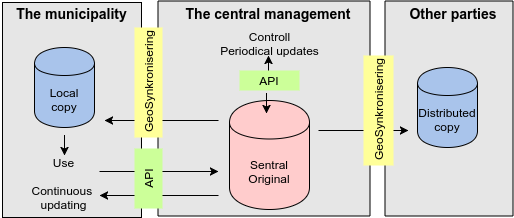
\includegraphics[scale=0.7]{img/consept.png}
%	\caption{Illustration of the concept of data distribution in the systems of both SFKB and the cadastre. The figure is adopted from \cite{Kartverket2015} }
%	\label{fig:konsept}
%\end{figure}
\begin{figure}[H]
	\centering
	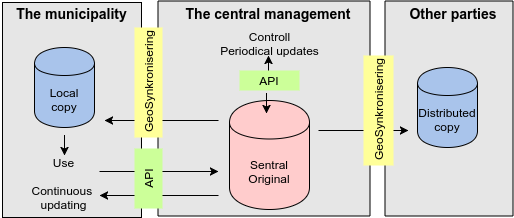
\includegraphics[scale=0.8]{img/consept.png}
	\caption{Illustration of the concept of data distribution in the systems of both SFKB and the cadastre. The figure is adapted from \cite{Kartverket2015} }
	\label{fig:konsept}
\end{figure}


%%=========================================
%\section{Plagiarism}

%\begin{quote}
%Two totally different cases, referred to as creep hypotheses $A$ and $B$, have been used as a basis of discussion to assess the effect of creep during the primary consolidation phase.
%\newline \mbox{} \hfill \citet{Deg2011Geo}
%\end{quote}
%&\end{itemize}



